
%aca va el ejercicio

Se tomaron los datos de máximos y mínimos de las entradas y salidas para los distintos estados de las hojas de datos de los circuitos en cuestiín, y se exhiben en el cuadro \ref{tab:datos74}.
\begin{table}[H]
\begin{tabular}{|l|l|l|l|l|l|l|}
\hline
                                                                            & Vcc                                                        & Voltage (25 C)                                              & Vcc         & Voltage (25 C) & Vcc      & Voltage (25 C)   \\ \hline
                                                                      & \multicolumn{2}{l|}{74HC02}                                                                                              & \multicolumn{2}{l|}{74HCT02} & \multicolumn{2}{l|}{74LS02} \\ \hline
\begin{tabular}[c]{@{}l@{}}Minimum HIGH Level\\ Input Voltage\end{tabular}  & \begin{tabular}[c]{@{}l@{}}2.0V\\ 4.5V\\ 6.0V\end{tabular} & \begin{tabular}[c]{@{}l@{}}1.5V\\ 3.15V\\ 4.2V\end{tabular} & 4.5V a 5.5V & 2V             & 4.75V    & 2V               \\ \hline
\begin{tabular}[c]{@{}l@{}}Maximum LOW Level\\ Input Voltage\end{tabular}   & \begin{tabular}[c]{@{}l@{}}2.0V\\ 4.5V\\ 6.0V\end{tabular} & \begin{tabular}[c]{@{}l@{}}0.5V\\ 1.35V\\ 1.8V\end{tabular} & 4.5V a 5.5V & 0.8V           & 4.75V    & 0.8V             \\ \hline
\begin{tabular}[c]{@{}l@{}}Minimum HIGH Level\\ Output Voltage\end{tabular} & \begin{tabular}[c]{@{}l@{}}2.0V\\ 4.5V\\ 6.0V\end{tabular} & \begin{tabular}[c]{@{}l@{}}1.9V\\ 4.4V\\ 5.9V\end{tabular}  & 4.5V a 5.5V & 4.4V           & 4.75V    & 2.7V             \\ \hline
\begin{tabular}[c]{@{}l@{}}Maximum LOW Level\\ Output Voltage\end{tabular}  & \begin{tabular}[c]{@{}l@{}}2.0V\\ 4.5V\\ 6.0V\end{tabular} & \begin{tabular}[c]{@{}l@{}}0.1V\\ 0.1V\\ 0.1V\end{tabular}  & 4.5V a 5.5V & 0.1V           & 4.75V    & 0.5V             \\ \hline
\end{tabular}
\caption{Tabla de informaciín obtenida de las hojas de datos}
\label{tab:datos74}
\end{table}

Como se ilustra en las figuras para los cuatro casos planteados, sílo habría problemas si se intenta conectar un transistor HC a la salida de un LS: la salida alta del LS puede caer en la regiín indeterminada de la entrada del HC, y sin que falle ningín componente fallaría el circuito.

En todos los demás casos se genera un margen de error para las entradas de los transistores.


%\begin{figure}[h]% este es para caption arriba o abajo
%  \centering
%    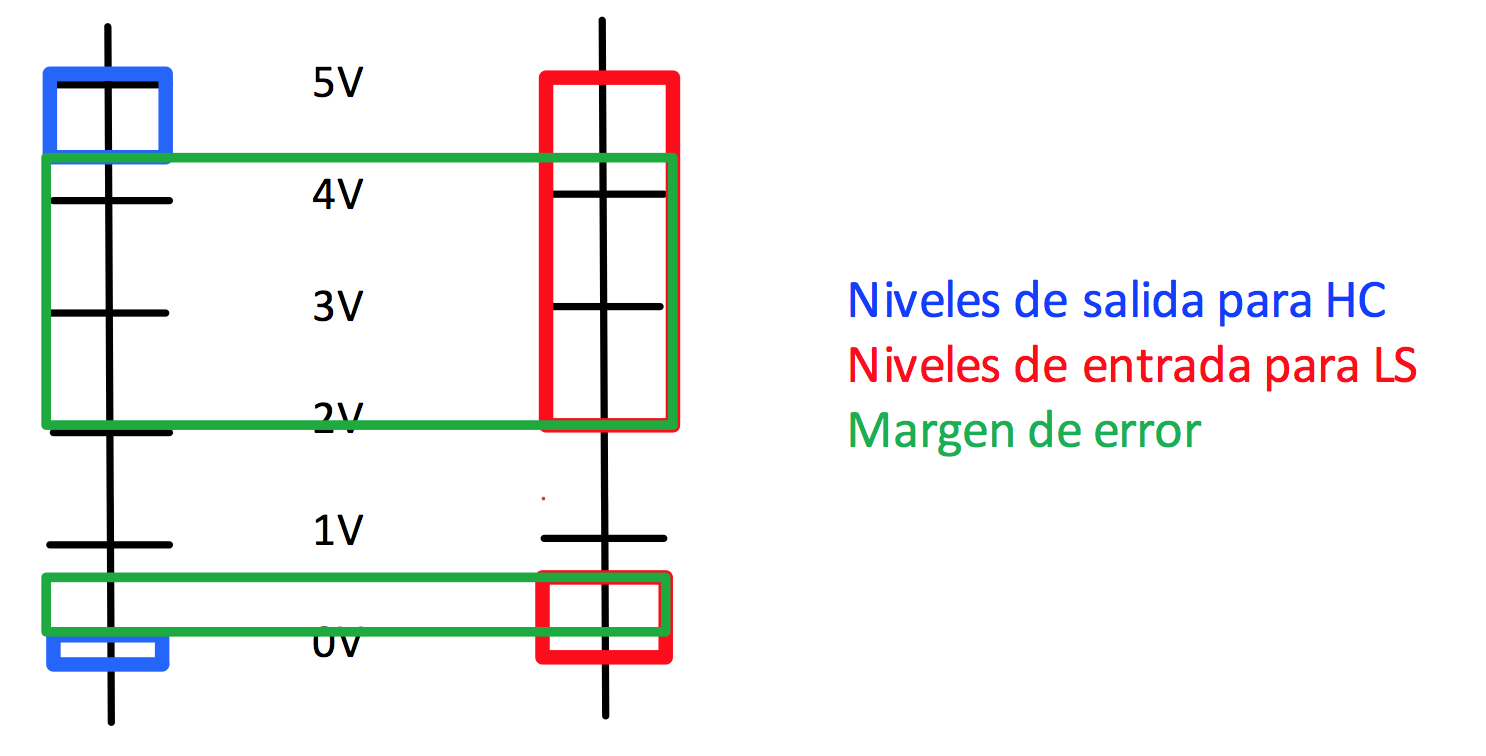
\includegraphics[width=0.5\textwidth]{HC->LS}
%    \caption{Niveles de tensiín para caso HC->LS.} %caption abajo
%\end{figure}
%
%\begin{figure}[h]% este es para caption arriba o abajo
%  \centering
%    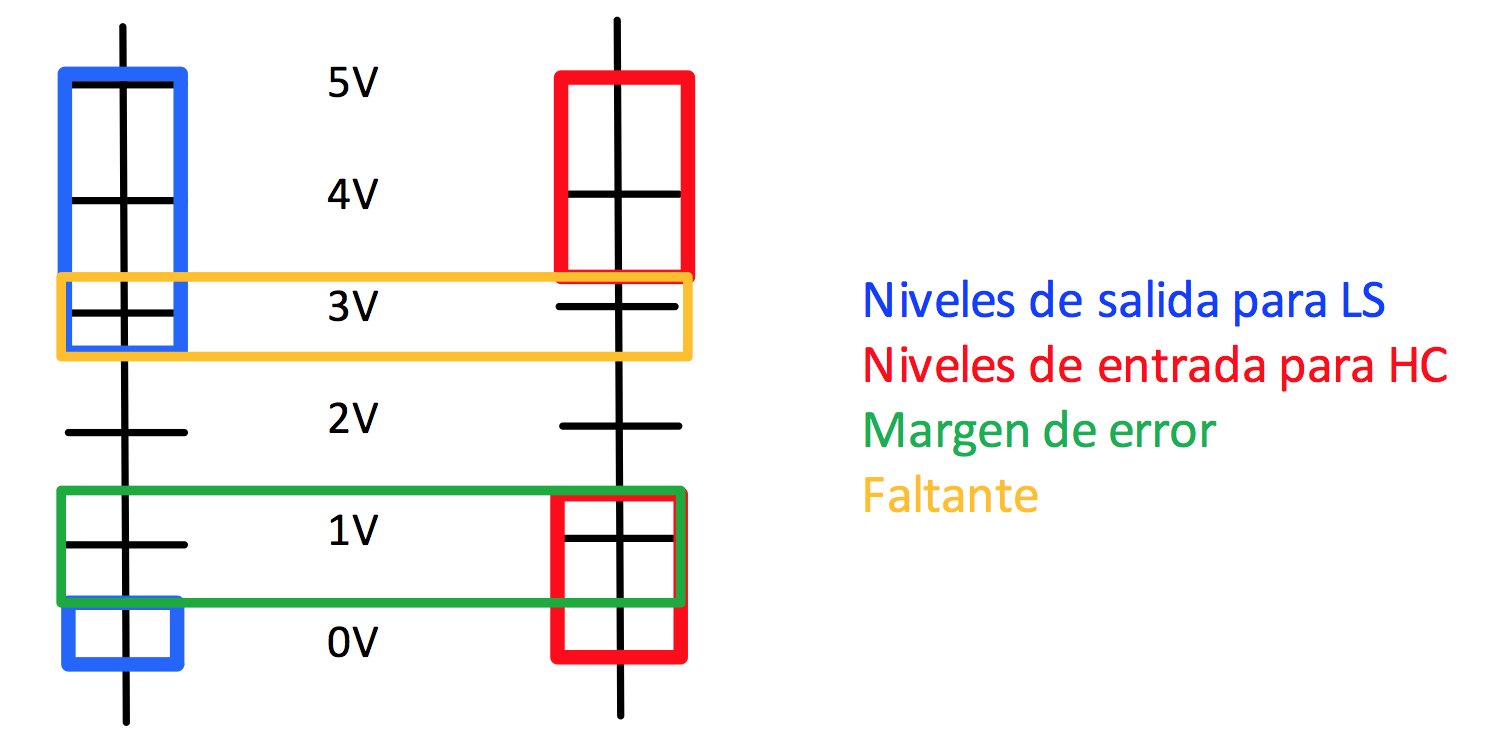
\includegraphics[width=0.5\textwidth]{LS->HC}
%    \caption{Niveles de tensiín para caso LS->HC.} %caption abajo
%\end{figure}
%
%\begin{figure}[h]% este es para caption arriba o abajo
%   \centering
%    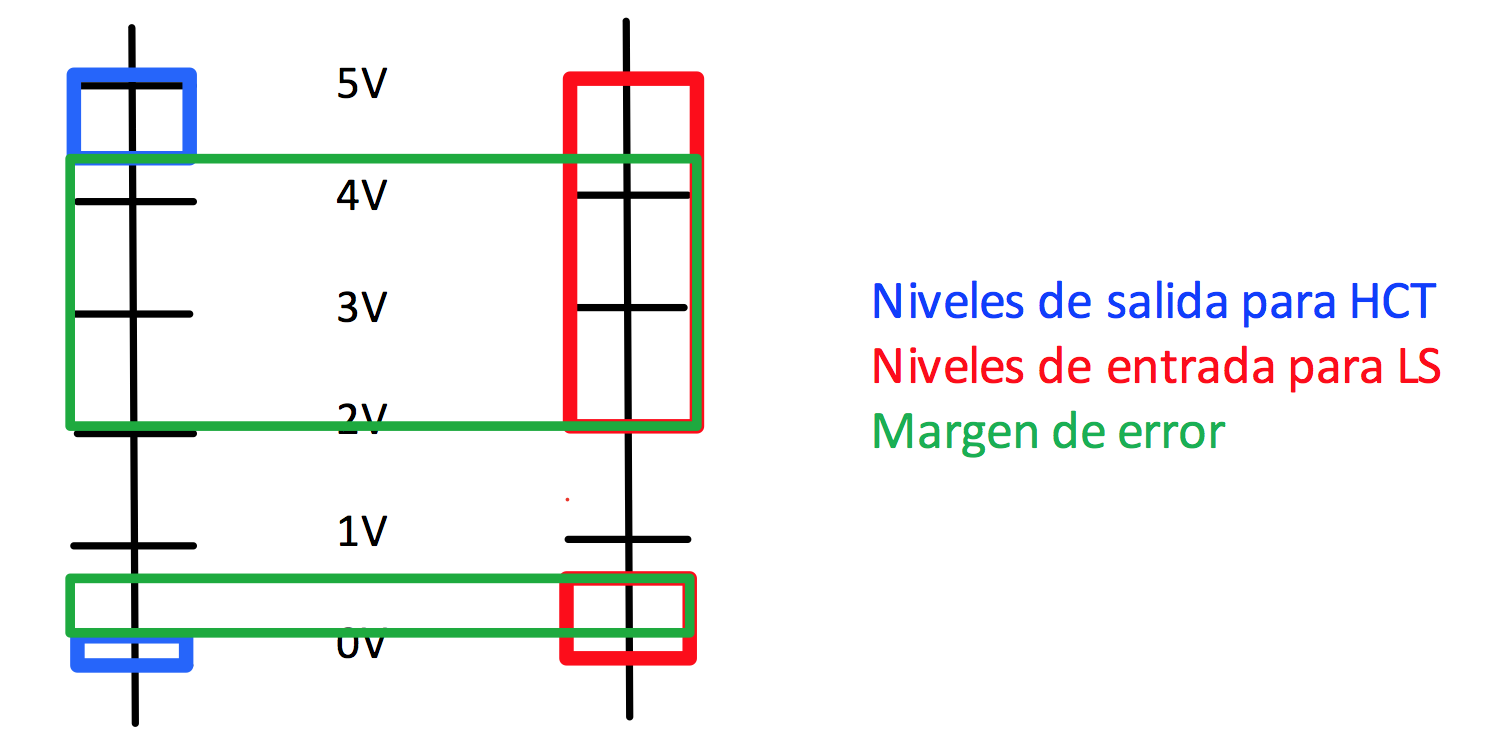
\includegraphics[width=0.5\textwidth]{HCT->LS}
%    \caption{Niveles de tensiín para caso HCT->LS.} %caption abajo
%\end{figure}
%
%\begin{figure}[h]% este es para caption arriba o abajo
%   \centering
%    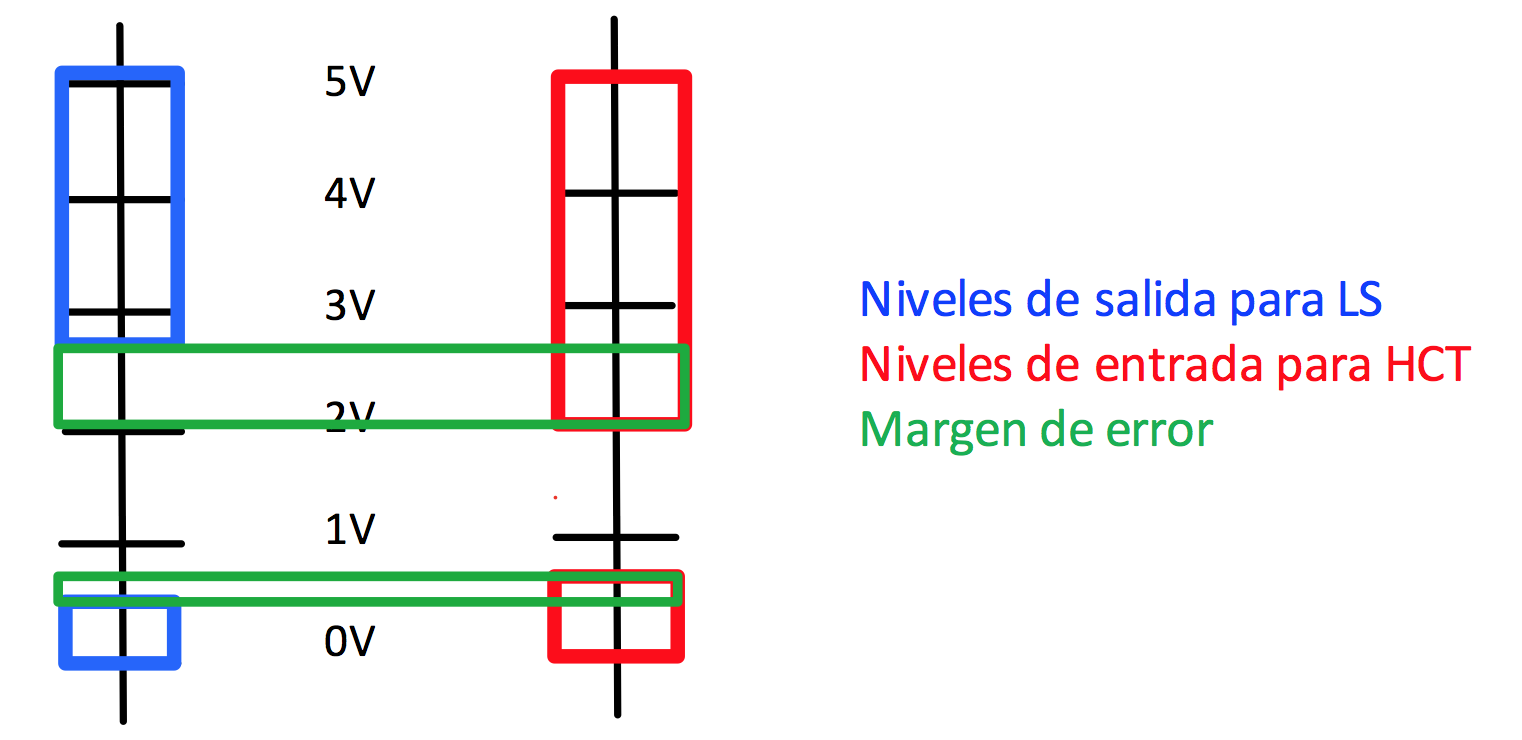
\includegraphics[width=0.5\textwidth]{LS->HCT}
%    \caption{Niveles de tensiín para caso LS->HCT.} %caption abajo
%\end{figure}

Procedimos a alimentar una compuerta del integrado LS02 con la salida de una misma compuerta pero del integrado HC02, y luego alimentamos de la misma manera pero en sentido inverso. Pudimos notar que hay zonas donde el circuito armado no debería andar de forma íptima por el margen de ruido que manejan las distintas compuertas pero funciona igual ya que la caída de tensiín en el LS02 no es tan grande y alcanza a caer cerca del límite del HC02 con 4,2V aproximadamente que es el mínimo del estado HIGH para el HC02. Si hubiera sido menor el valor de la tensiín no hubiíramos obtenido alguna salida por lo marcado en las hojas de datos.
\newline
El \textbf{fan-out} está determinado por la cantidad de corriente que puede aceptar en la entrada cada CI y es la cantidad de pines que puede alimentar un CI con alguna de sus salidas. En la tecnología CMOS(HC) segín su hoja de dato acepta 20mA como máximo, mientras que la tecnología TTL(LS) acepta 0,4mA como máximo en la entrada y 8mA en la salida. Haciendo las cuentas directas de estos casos, con la salida de un integrado LS puedo alimentar hasta 20 entradas LS, mientras que con un HC puedo alimentar 50 entradas LS. Cabe destacar que en la hoja de datos que brinda el fabricante solo asegura el funcionamiento de hasta 10 pines LS-TTL con una salida del HC, el cual debe ser para el peor caso que puede surgir para este integrado.
\newline
Al hacer las mediciones alimentando con el HCT y notamos un comportamiento mejor en cuanto la alimentaciín del LS02, ya que la tecnología HCT es a base de CMOS pero tiene una gran tolerancia con la tecnología TTL en cuanto a los valores de tensiín.